% document formatting
\documentclass[10pt]{article}
\usepackage[utf8]{inputenc}
\usepackage[left=1in,right=1in,top=1in,bottom=1in]{geometry}
\usepackage[T1]{fontenc}
\usepackage{xcolor}

% math symbols, etc.
\usepackage{amsmath, amsfonts, amssymb, amsthm}

% lists
\usepackage{enumerate}

% images
\usepackage{graphicx} % for images

% code blocks
\usepackage{minted, listings} 

% verbatim greek
\usepackage{alphabeta}

\graphicspath{{./assets/images}}

\newcommand{\solution}{\textbf{Solution:}} 
\newcommand{\example}{\textbf{Example: }}
\newcommand{\R}{\mathbb{R}}

\title{COM SCI 122 Week 4}

\author{Aidan Jan}
\date{\today}

\begin{document}
\maketitle

\section*{Graph Algorithms in Bioinformatics}
\subsection*{Introduction}
A \textbf{graph} is a collection (V, E) of two sets:
\begin{itemize}
    \item V is simply a set of objects, which we call the \textbf{vertices} of G.
    \item E is a set of pairs of vertices which we call the \textbf{edges} of G.
\end{itemize}
Simpler: Think of G as a network:
\begin{itemize}
    \item Nodes = vertices
    \item Edges = segments connecting the nodes
\end{itemize}
\begin{center}
    \includegraphics*[scale=0.8]{W4_1.png}
\end{center}

\section*{Hamiltonian Cycle Problem}
\begin{itemize}
    \item Input: A graph G = (V, E)
    \item Output: A \textbf{Hamiltonian cycle} in G, which is a cycle that visits every vertex exactly once.
    \item This problem is NP-Complete.
    \begin{itemize}
        \item This result explains why knight tours were so difficult to find; there is no known quick method to find them!
    \end{itemize}
\end{itemize}

\subsection*{Traveling Salesman Problem (TSP)}
\begin{itemize}
    \item $n$ cities
    \item Cost of traveling from $i$ to $j$ is given by c($i, j$)
    \item Goal: Find the tour of all the cities of lowest total cost
    \item Example below: One busy salesman!
\end{itemize}
\begin{center}
    \includegraphics*[scale=0.9]{W4_2.png}
\end{center}
So we might like to think of the Hamiltonian Cycle Problem as a TSP with all costs = 1, where we have some edges missing (there doesn't always exist a flight between all pairs of cities).

\subsection*{The Bridges of Konigsberg}
\begin{itemize}
    \item The city of Konigsberg, Prussia (today: Kaliningrad, Russia) was made up of both banks of a river, as well as two islands.
    \item The riverbanks and the islands were connected with bridges, as follows:
    \begin{center}
        \includegraphics*[scale=0.9]{W4_3.png}
    \end{center}
    \item The residents wanted to know if they could take a walk from anywhere in the city, cross each bridge exactly once, and wind up where they started.
\end{itemize}
In 1735, enter Euler\dots his idea: compress each land area down to a single point, and each bridge down to a segment connecting two points.  This is just a graph!  We are now looking for a cycle in this graph which covers each edge exactly once.\\\\
Using this setup, Euler showed that such a cycle cannot exist.

\subsection*{Eulerian Cycle Problem}
\begin{itemize}
    \item Input: A graph G = (V, E)
    \item Output: A cycle in G that touches every edge in E (called an \textbf{Eulerian cycle}), if one exists.
    \item Example: below is a demonstration of an Eulerian cycle.
\end{itemize}
\begin{center}
    \includegraphics*[scale=0.8]{W4_4.png}
\end{center}

\subsubsection*{Theorem:}
The Eulerian Cycle Problem can be solved in linear time
\begin{itemize}
    \item So whereas finding a Hamiltonian cycle quickly becomes intractable for an arbitrary graph, finding an Eulerian cycle is relatively much easier
\end{itemize}

\subsection*{Shortest Superstring Problem (SSP)}
\begin{itemize}
    \item Problem: Given a set of strings, find a shortest string that contains all of them,
    \item Input: Strings $s_1$, $s_2$, \dots, $s_n$
    \item Output: A "superstring" $s$ that contains all strings $s_1$, $s_2$, \dots, $s_n$ as substrings, such that the length of $s$ is minimized.
\end{itemize}

\subsubsection*{Example:}
\begin{center}
    \includegraphics*[scale=0.8]{W4_5.png}
\end{center}
\begin{itemize}
    \item So our greedy guess of concatenating all the strings together turns out to be substantially suboptimal (length 24 vs. 10).
\end{itemize}
To do this, we can define an \textit{overlap function}.

\subsubsection*{Overlap Function}
\begin{itemize}
    \item Given strings $s_i$ and $s_j$, define $overlap(s_i, s_j)$ as the length of the longest prefix of $s_j$ that matches a suffix of $s_i$.
    \item Example:
    \begin{verbatim}
        s_1 = AAAGGCATCAAATCTAAAGGCATCAAA
        s_2 =                AAAGGCATCAAATCTAAAGGCATCAAA
    \end{verbatim}
    \begin{itemize}
        \item Therefore, $overlap(s_1, s_2) = 12$.
    \end{itemize}
\end{itemize}

\subsection*{Why is SSP an NP-Complete Problem?}
\begin{itemize}
    \item Construct a graph G as follows:
    \begin{itemize}
        \item The $n$ vertices represent the $n$ strings $s_1, s_2, \dots, s_n$.
        \item For every pair of vertices $s_i$ and $s_j$, insert an edge of length $overlap(s_i, s_j)$ connecting the vertices.
    \end{itemize}
    \item Then finding the shortest superstring will correspond to finding the shortest Hamiltonian path in G.
    \item But this is the \textbf{Traveling Salesman Problem} (TSP), which we know to be NP-complete.
    \begin{itemize}
        \item Hence SSP must also be NP-complete!
    \end{itemize}
\end{itemize}

\subsection*{Reducing SSP to TSP: Example 1}
\begin{itemize}
    \item Take our previous set of strings S = \{000, 001, 010, 011, 100, 101, 110, 111\}
    \item Then the graph for S is below:
    \begin{center}
        \includegraphics*[scale=0.8]{W4_6.png}
    \end{center}
    \item One minimal Hamiltonian path gives our previous superstring, 0001110100.    
\end{itemize}

\subsection*{Reducing SSP to TSP: Example 2}
\begin{itemize}
    \item S = \{ATC, CCA, CAG, TCC, AGT\}
    \item This graph is provided below.
    \begin{center}
        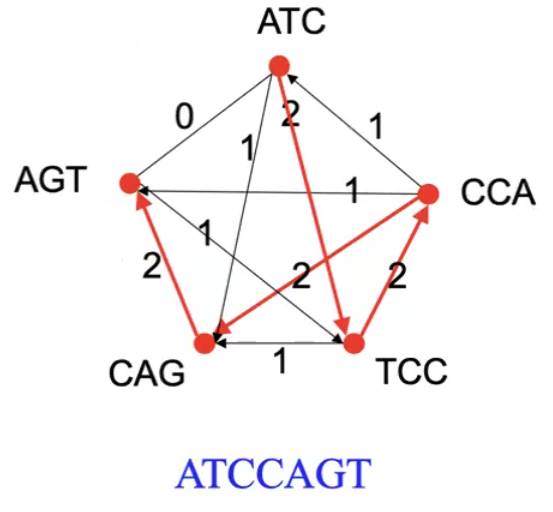
\includegraphics[scale=0.8]{W4_7.png}
    \end{center}
    \item A minimal Hamiltonian path gives as shortest superstring ATCCAGT.
\end{itemize}

\section*{Sequencing By Hybridization}
\begin{itemize}
    \item Using a spectroscopic detector, determine which probes hybridize to the DNA fragment to obtain the $l$-mer composition of the target DNA fragment.
    \item Reconstruct the sequence of the target DNA fragment from the $l$-mer composition.
\end{itemize}
\begin{center}
    \includegraphics*[scale=0.6]{W4_8.png}
\end{center}

\subsection*{How SBH Works: Example}
\begin{itemize}
    \item Say our DNA fragment hybridizes to indicate that it contains the following substrings: GCAA, CAAA, ATAG, TAGG, ACGC, GGCA.
    \item Then the most logical explanation is that our fragment is the shortest superstring containing these strings!
    \item Here the superstring is: ATAGGCAAACGC.
\end{itemize}
\begin{center}
    \includegraphics*[scale=0.8]{W4_9.png}
\end{center}

\subsection*{$l$-mer Composition}
\begin{itemize}
    \item $Spectrum(s, l)$: The \textit{unordered} of all $l$-mers in a string $s$ of length $n$.
    \item The order of individual elements in $Spectrum(s, l)$ does not matter.
    \item For $s$ = TATGGTGC all of the following are equivalent representations of $Spectrum(s, 3)$:
    \begin{itemize}
        \item \{TAT, ATG, TGG, GGT, GTG, TGC\}
        \item \{\textcolor{red}{ATG, GGT, GTG, TAT, TGC, TGG}\}
        \item \{TGG, TGC, TAT, GTG, GGT, ATG\}
    \end{itemize}
    \item Which ordering do we choose?  Typically the one that is \textit{lexicographic}, meaning in alphabetical order (think of a phonebook).
\end{itemize}

\subsubsection*{Different Sequences, Same Spectrum}
\begin{itemize}
    \item Different sequences may share a common spectrum
    \item Example:
    \begin{center}
        \includegraphics*[scale=0.8]{W4_10.png}
    \end{center}
\end{itemize}

\subsection*{The SBH Problem}
\begin{itemize}
    \item Problem: Reconstruct a string from its $l$-mer composition
    \item Input: A set $S$, representing all $l$-mers from an (unknown) string $s$
    \item Output: A string $s$ such that $Spectrum(s, l) = S$
    \item \textbf{Note:} As we have seen, there may be more than one correct answer.  Determining which DNA sequence is actually correct is another matter.
\end{itemize}

\subsubsection*{SBH: Hamiltonian Path Approach}
\begin{itemize}
    \item Create a graph G as follows:
    \begin{itemize}
        \item Create one vertex for each member of $S$.
        \item Connect vertex $v$ to vertex $w$ with a \textit{directed} edge (arrow) if the last $l - 1$ elements of $v$ match the first $l - 1$ elements of $w$.
    \end{itemize}
    \item Then a Hamiltonian path in this graph will correspond to a string $s$ such that $Spectrum(s, l)$!
\end{itemize}
\textbf{Example:}
\begin{center}
    \includegraphics*[width=\textwidth]{W4_11.png}
\end{center}
\begin{itemize}
    \item There are actually two Hamiltonian paths in this graph:
    \begin{itemize}
        \item Path 1: Gives the string $S$ = ATGCGTGGCA
        \item Path 2: Gives the string $S$ = ATGGCGTGCA
    \end{itemize}
\end{itemize}

\subsubsection*{SBH: A Lost Cause?}
\begin{itemize}
    \item At this point, we should be concerned about using a Hamiltonian path to solve SBH.
    \item After all, recall that SSP was an NP-Complete problem, and we have seen that an instance of SBH is an instance of SSP.
    \item However, note that SBH is actually a specific case of SSP, so there is still hope for an efficient algorithm for SBH:
    \begin{itemize}
        \item We are considering a spectrum of only $l$-mers, and not strings of any other length.
        \item Also, we only are connecting two $l$-mers with an edge if and only if the overlap between them is $l$ - 1, whereas before we connected $l$-mers if there was any overlap at all.
    \end{itemize}
    \item \textbf{Note:} SBH is not NP-Complete since SBH reduces to SSP, but not vice versa.
\end{itemize}

\subsubsection*{SPH: Eulerian Path Approach}
\begin{itemize}
    \item So instead, let us consider a completely \textit{different} graph G:
    \begin{itemize}
        \item Vertices = the set of ($l - 1$)-mers which are substrings of some $l$-mer from our set $S$.
        \item $v$ is connected to $w$ with a \textit{directed} edge if the final $l - 2$ elements of $v$ agree with the first $l - 2$ elements of $w$, and the \textit{union} of $v$ and $w$ is in $S$.
    \end{itemize}
    \item \textbf{Example:} $S$ = \{ATG, TGG, TGC, GTG, GGC, GCA, GCG, CGT\}
    \begin{itemize}
        \item V = \{AT, TG, GG, GC, GT, CA, CG\}
        \item E = shown below.
    \end{itemize}
    \begin{center}
        \includegraphics*[scale=0.8]{W4_12.png}
    \end{center}
    \item \textbf{Key Point:} A sequence reconstruction will actually correspond to an \textit{Eulerian} path in this graph
    \item Recall that an Eulerian path is "easy" to find (one can always be found in linear time)... so we have found a simple solution to SBH!
    \item In our example, two solutions: 
    \begin{itemize}
        \item ATGGCGTGCA
        \item ATGCGTGGCA
    \end{itemize}
\end{itemize}

\subsubsection*{But, How do we know an Eulerian Path exists?}
\begin{itemize}
    \item A graph is \textbf{balanced} if for every vertex the number of incoming edes equals to the number of outgoign edges.  We write this for vertex $v$ as:
    \[in(v) = out(v)\]
    \item \textbf{Theorem:} A connected graph is \textit{Eulerian} (i.e., contains an Eulerian cycle) if and only if each of its vertices is balanced.
    \item We will prove this be demonstrating the following:
    \begin{enumerate}
        \item Every Eulerian graph is balanced.
        \item Every balanced graph is Eulerian.
    \end{enumerate}
\end{itemize}

\subsubsection*{Proof: Every Eulerian Graph is Balanced}
\begin{itemize}
    \item Suppose we have an Eulerian graph G.  Call $C$ the Eulerain cycle of G, and let $v$ be any vertex of G.
    \item For every edge $e$ entering $v$, we can pair $e$ with an edge leaving $v$, which is simply the edge in our cycle $C$ that follows $e$.
    \item Therefore, it directly follows that $in(v) = out(v)$ as needed, and since our choice of $v$ was arbitrary, this relation must hold for all vertices in G, so we are finished with the first part.
\end{itemize}

\subsubsection*{Proof: Every Balanced Graph is Eulerian}
\begin{itemize}
    \item Next, suppose that we have a balanced graph G.
    \item We will actually \textit{construct} an Eulerian cycle in G.
    \item Start with an arbitrary vertex $v$ and form a path in G without repeated edges until we reach a "dead end," meaning a vertex with no unused edges leaving it.
    \item G is balanced, so every time we enter a vertex $w$ that isn't $v$ during the course of our path, we can find an edge leaving $w$.  So our dead end is $v$ and we have a \textit{cycle}.
    \item We have two simple cases for our cycle, which we call C:
    \begin{enumerate}
        \item C is an Eulerian cycle $\rightarrow$ G is Eulerian $\rightarrow$ DONE.
        \item C is not an Eulerian cycle.
    \end{enumerate}
    \item So we can assume that C is not an Eulerian cycle, which means that C contains vertices which have untraversed edges.
    \item Let $w$ be such a vertex, and start a new path from $w$.  Once again, we must obtain a cycle, say C'.
    \item Combine our cycles C and C' into a bigger cycle C$^*$ by swapping edges at $w$.
    \item Once again, we test C$^*$:
    \begin{enumerate}
        \item C$^*$ is an Eulerian cycle $\rightarrow$ G is Eulerian $\rightarrow$ DONE
        \item C$^*$ is not an Eulerian cycle.
    \end{enumerate}
    \item If C$^*$ is not Eulerian, we iterate our procedure.  Because G has a finite number of edges, we must eventually reach a point where our current cycle is Eulerian (Case 1 above).  DONE.
\end{itemize}

\subsection*{Euler's Theorem: Extension}
\begin{itemize}
    \item A vertex $v$ is \textbf{semi-balanced} if either $in(v) = out(v) + 1$ or $in(v) = out(v) - 1$.
    \item \textbf{Theorem:} A connected graph has na Eulerian path if and only if it contains at most two semi-balanced vertices and all other vertices are balanced.
    \begin{itemize}
        \item If G has no semi-balanced vertices, DONE.
        \item If G has two semi-balanced vertices, connect them with a new edge, $e$, so that the graph G + $e$ is balanced and must be Eulerian.  Remove $e$ from the Eulerian cycle in G + $e$ to obtain an Eulerian path in G.
    \end{itemize}
    \item \textbf{Think:} Why can G not have just one semi-balanced vertex?
\end{itemize}

\subsection*{Some Difficulties with SBH}
\begin{itemize}
    \item \textbf{Fidelity of Hybridization:} It is difficult to detect differences between probes hybridized with perfect matches and those with one mismatch
    \item \textbf{Array Size:} The effect of low fidelity can be decreased with longer $l$-mers, but array size increases exponentially in $l$.  Array size is limited with current technology.
    \item \textbf{Practicality:} SBH is still impractical.  As DNA microarray technology improves, SBH may become practical in the future.
    \item \textbf{Practicality Again:} Although SBH is still impractical, it spearheaded expression analysis and SNP analysis techniques.
    \item \textbf{Practicality Again and Again:} In 2007 Solexa (now Illumina) developed a new DNA sequencing approach that generates so many short $l$-mers that they essentially mimic a universal DNA array.
\end{itemize}

\section*{Fragment Assembly and Repeats in DNA}
\subsection*{Shotgun Sequencing}
\begin{center}
    \includegraphics*[width=\textwidth]{W4_13.png}
\end{center}

\subsection*{Challenges in Fragment Assembly}
\begin{itemize}
    \item Repeats: A \textbf{major} problem for fragment assembly
    \item More than 50\% of human genome are repeats:
    \begin{itemize}
        \item Over 1 million \textit{Alu} repeats (about 300 bp)
        \item About 200,000 LINE repeats (1000 bp and longer)
    \end{itemize}
\end{itemize}
\begin{center}
    \includegraphics*[width=\textwidth]{W4_14.png}
\end{center}

\subsection*{Overlap Graph: Hamiltonian Approach}
\begin{itemize}
    \item Each vertex represents a read from the original sequence.
    \item Vertices are connected by an edge if they overlap.
    \begin{center}
        \includegraphics*[width=\textwidth]{W4_15.png}
    \end{center}
    \item So finding an alignment corresponds to finding a Hamiltonian path in the overlap graph.
    \item Recall that the Hamiltonian path/cycle problem is \textit{NP-Complete}: no efficient algorithms are known.
\end{itemize}

\subsection*{Euler Approach to Fragment Assembly}
\begin{itemize}
    \item The "overlap-layout-consensus" technique implicitly solves the Hamiltonian path problem and has a high rate of mis-assembly.
    \item Can we adapt the Eulerian Path approach borrowed from the SBH problem?
    \item Fragment assembly without repeat masking can be done in linear time with greater accuracy.
\end{itemize}

\subsection*{Repeat Graph: Eulerian Approach}
\begin{center}
    \includegraphics*[width=\textwidth]{W4_16.png}
\end{center}

\subsection*{Making Repeat Graph from Reads Only}
\begin{itemize}
    \item \textbf{Problem:} In previous slides, we have constructed the repeat graph while \textit{already knowing} the genome structure.
    \item How do we construct the repeat graph just from fragmets?
    \item \textbf{Solution:} Break the reads into smaller pieces.
\end{itemize}
\begin{center}
    \includegraphics*[width=\textwidth]{W4_17.png}
\end{center}

\subsection*{Repeat Sequences: Emulating a DNA Chip}
\begin{itemize}
    \item A virtual DNA chip allows one to solve the fragment assembly problem using our SBH algorithm.
\end{itemize}
\begin{center}
    \includegraphics*[width=\textwidth]{W4_18.png}
\end{center}

\subsection*{Construction of Repeat Graph}
\begin{itemize}
    \item \textbf{Construction of Repeat Graph from $k$-mers}: emulates an SBH experiment with a huge (virtual) DNA chip.
    \item \textbf{Breaking reads into $k$-mers}: Transforms sequencing data into virtual DNA chip data.
    \item Error correction in reads: "Consensus first" approach to fragment assembly.
    \begin{itemize}
        \item Makes reads (almost) error-free BEFORE the assembly even starts.
    \end{itemize}
    \item Uses reads and mate-pairs to simplify the repeat graph (Eulerian Superpath Problem.)
\end{itemize}

\subsection*{Practical Sequence Assembly}
\begin{itemize}
    \item Split reads into kmers
    \item Error correct kmers based on occurrence threshold
    \item Construct De Bruijn Graph (Eulerian Graph)
    \item Find Eulerian Path (or as many long paths as possible)
\end{itemize}


\end{document}